
\documentclass[11pt]{article}

\usepackage[utf8]{inputenc}
\usepackage[ngerman]{babel}
\usepackage{csquotes}

\usepackage{fullpage}
\usepackage{setspace}
\usepackage{parskip}
\usepackage{titlesec}
\usepackage{mathptmx}
\usepackage{comment}

\usepackage{graphicx}
\usepackage[section]{placeins}
\usepackage[justification=centering]{caption}
\usepackage{wrapfig}
\usepackage{subfigure}

\usepackage{authblk}
\usepackage{hyperref}


\PassOptionsToPackage{
style=apa,
doi=false,
isbn=false,
eprint=false
}{biblatex}
\usepackage[backend=biber]{biblatex}
\addbibresource{ws1819_skribbl.bib}

\PassOptionsToPackage{hyphens}{url}

\makeatletter

\renewenvironment{abstract}
{{\bfseries\noindent{\abstractname}\par\nobreak}\footnotesize}
{\bigskip}

\renewenvironment{quote}
  {\begin{tabular}{|p{13cm}}}
  {\end{tabular}}

\titlespacing{\section}{0pt}{*3}{*1}
\titlespacing{\subsection}{0pt}{*2}{*0.5}
\titlespacing{\subsubsection}{0pt}{*1.5}{0pt}

\begin{document}

\begin{titlepage}
   \begin{center}
       \vspace*{1cm}

       \Huge
       Skribbl.AI Projektdokumentation (IQ vs. KI)
       \vspace{1.5cm}

       
\includegraphics[width=0.4\textwidth]{images/logo_htw.jpg}

       \vspace{1.0cm}
       
\includegraphics[width=0.2\textwidth]{images/logo_skribbl.png}
       \vspace{1.0cm}

       \LARGE

       Josefine Sophie Busch, Malin Dulkies, Rachel Escueta, Tim-Niklas Heise, Ninoslav Kjireski, Anastasiia Litvina, Anh Quang Vu-Tuyen

       \vfill

       Projektarbeit \\

       \vspace{0.8cm}

       Hochschule für Technik und Wirtschaft\\
       Berlin\\

       Prof. Dr. Klaus Jung\\
       Wintersemester 2018/2019\\
       
	\end{center}
\end{titlepage}
\pagenumbering{roman}
\pagebreak
\tableofcontents
\pagebreak
\listoftables
\listoffigures
\pagebreak
\pagenumbering{arabic}
\section{Einleitung}
\label{chap: Einleitung}
\subsection{Leitfaden}
\label{chap: leitfaden}
\begin{wrapfigure}{R}{0.3\textwidth}
\centering

\includegraphics[width=0.25\textwidth]{images/logo_skribbl.png}
\caption{\label{fig:skribblLogo}Skribbl.AI Logo}
\end{wrapfigure}
Die Idee begann mit IQ gegen KI. Mit dem Einfall, was würde eigentlich passieren, wenn eine künstliche Intelligenz ein von einem Menschen gemaltes Bild  erkennen sollte? \\
Neuronale Netzwerke erbringen beeindruckende Leistungen bei der Erkennung fotorealistischer Aufnahmen. Sie helfen sogar Pathologen bei der Erkennung von Krebszellen \parencite{ElizabethDougherty2018}.\\
Was also würde  passieren, wenn wir eine künstliche Intelligenz mit den Kritzeleien einer Student*in konfrontieren?
 
\subsection{Aufbau des Projektes}
\label{chap: Aufbau}

Das Semesterprojekt ist ein Pflichtmodul des Studiengang Internationale Medieninformatik der HTW Berlin, welches im 5. Semester angesetzt ist. \\
In einer Gruppe von fünf bis acht zufällig gewählten Studierenden werden Konzepte entwickelt und dann in Anwendungen umgesetzt. Dabei stehen Themen aus Bereichen der Wirtschaft oder aus einem der verschiedenen Forschungsbereiche des Studienganges zur Wahl, an denen die Studierenden arbeiten können.

Die Studierenden werden dabei von einer Lehrkraft bzw. einer verantwortlichen Person aus dem wirtschaftlichen Unternehmen betreut.
Das Projekt ist in drei Bereiche unterteilt.

\subsubsection{ Themenvergabe und Konzeptausarbeitung }
\label{chap: Themenvergabe}

Unser Projekt ist das Projekt KI vs IQ, welches von Prof. Jung betreut wurde.
Die Vorgabe war, eine spielerische Anwendung zu entwickeln, in der ein Mensch gegen ein neuronales Netz antritt, welches dazu trainiert wurde, Bilder zu erkennen.\\
Mehr dazu in \autoref{chap: Grundlagen}
	
\subsubsection{  Projektmanagement }
\label{chap: Projektmanagement}
Die Belegung des Semesterprojektes erfolgt mit einer automatischen Belegung des Projektmanagement Moduls, welches agile Methoden im Allgemeinen und Scrum im Speziellen vermittelt. Dem entsprechend und der Tatsache zugrundeliegend, dass einige Gruppenmitglieder bereits Erfahrung mit Scrum hatten, haben wir uns dafür entschieden, im Projekt mit Scrum zu arbeiten beziehungsweise mit einer unseren Bedürfnissen und Gegebenheiten angepassten Version von Scrum.\\
Als unterstützende Werkzeuge für das Projektmanagement haben wir Trello und zum Gruppenmanagement beziehungsweise für die Kommunikation in der Gruppe Slack genutzt.

\subsubsection{ Durchführung }
\label{chap: durchfuhrung}
Die Durchführungsphase setzt sich dann konkret mit der Entwicklung der Anwendung auseinander. Wir entschieden uns dafür eine Website für unser Spiel zu bauen. Wir haben HTML 5, CSS 3, Sass 1.16.1 und Javascript (ECMAScript 6) für das entwickeln der Webumgebung und des Spieles genutzt. Das neuronale Netzwerk ist ein TensorFlow 1.12.0 Model mit Keras 2.2.2, welches wir mit TensorFlow.js in unsere Webseite einbinden und mit Python 3 trainieren.\\
Mehr dazu in \autoref{chap: Anforderungen}

\section{Grundlagen}
\label{chap: Grundlagen}
\subsection{Design}
\subsubsection{Findung und Sketcher}

Wissend, dass wir ein Spiel kreieren wollten, welches sowohl Bilderkennung durch ein neuronales Netzwerk garantiert als auch den Spielspaß für den Spieler, galten unsere ersten Überlegungen dem Namen sowie Konzept des Spiels.
Abgeleitet von dem englischen Verb 'to scribble' mit ein paar Änderungen um den Namen für das deutsche Publikum besser aussprechbar zu machen, wurde 'Skribbl'. Das Kürzel '.AI' hingegen war für uns als Team sehr offensichtlich. Nicht nur wäre es eine wundervolle URL, sollte das Projekt zu einem späteren Zeitpunkt veröffentlicht werden, sondern sie zeigt ebenfalls die nahe Verbindung zu unserem neuronalen Netzwerk.

Folgend kam die Entscheidung dahingehend, was für eine Art von Spiel wir erschaffen wollten. Eine Zeichnung sollte erkannt werden. Natürlich gab es zahlreiche Konzeptideen, so mussten wir uns auf ein Konzept einigen. Dabei hatten wir von Anfang an direkt 3 verschiedene Implementierungen, die uns einfielen. Alle angelehnt an das selbe Konzept und dennoch von Grund auf verschieden, was den Spielspaß anging. Sollten die Spieler sehen, welche Ergebnisse das neuronale Netz aus der Zeichnung vorhersagte, oder sollten sie komplett im Dunklen stehen? Sollte es eine Überraschung werden oder nicht? Vielleicht etwas in der Mitte?

Während der Anfangsphase des Projektes und bei der Rechercher stießen wir auf ähnliche Konzepte, die ebenfalls eine Bilderkennung mit Zeichnungen implementierten. Besonders hervorzuheben wären hier Sketcher \parencite{ZaidAlyafeai2018}, welches eine große Hilfe und Inspiration für uns war. Besonders hilfreich war auch das Tutorial von Zaid Alyafeai zu Sketcher \parencite{ZaidAlyafeaia}. Außerdem gibt es auch ein Projekt von Google \parencite{Google}.

\subsubsection{Mobile First}

Ein solches Projekt, mit Spiel-Charakter, wie man sie aus jedem App-Store kennt; kurze Level für ein Kurzweiliges Spielerlebnis machten eines schnell klar: Unsere Priorität lag auf Mobile-First.
Dabei mussten mögliche Hürden mit dem Touchscreen, den unterschiedlichen Bildschirmgrößen sowie Funktionen der verschiedenen Browser und Betriebssysteme erwartet werden. Dennoch war es für uns keine schwere Entscheidung den Desktop vorerst außen vor zu lassen und sicher zu stellen, dass unser Spiel optimal auf einem Smartphone spielbar ist.

\subsubsection{Accessibility}

Accessibility war ein Punkt, der zwar erst ein wenig später in unserem Projekt angesprochen wurde, aber dennoch von hoher Bedeutung für uns war. Mit dem sehr visuellen Thema des Zeichnens und der heutigen Einstellung zu Accessibility Themen, war uns schnell klar, dass wir unser Spiel so zugänglich wie möglich für alle Nutzer machen wollten.

Ein Styleguide wurde erstellt, in welchem jede Farbe und Schriftgröße so getestet wurde, dass sie den Werten des AA Standards der W3C Verordnung entspricht. Außerdem nahmen wir noch andere Richtlinen wie Clean Coding Regeln in unseren Styleguide mit auf.\\
Mehr dazu in \autoref{chap: Anlagen} 

\subsection{Layout}
Im Layout unseres Spiels haben wir möglichst minimalistisch gearbeitet und uns an die vier ausgewählten Hauptfarben gehalten. Durch das Responsive Design passt sich unser Layout an die Größe des Bildschirms beziehungsweise den Viewport an. Vorrangig haben wir das Layout für mobile Geräte in vertikaler Ausrichtung entwickelt. Durch die kleine Bildschirmgröße eine Smartphones würde das Zeichenerlebnis in horizontaler Ausrichtung leiden. Bei Tablets hingegen ist je nach Größe des Geräts auch das Spielen im Landscapemodus möglich.

\subsubsection{Startbildschirm}

\begin{wrapfigure}{R}{0.3\textwidth}
\centering
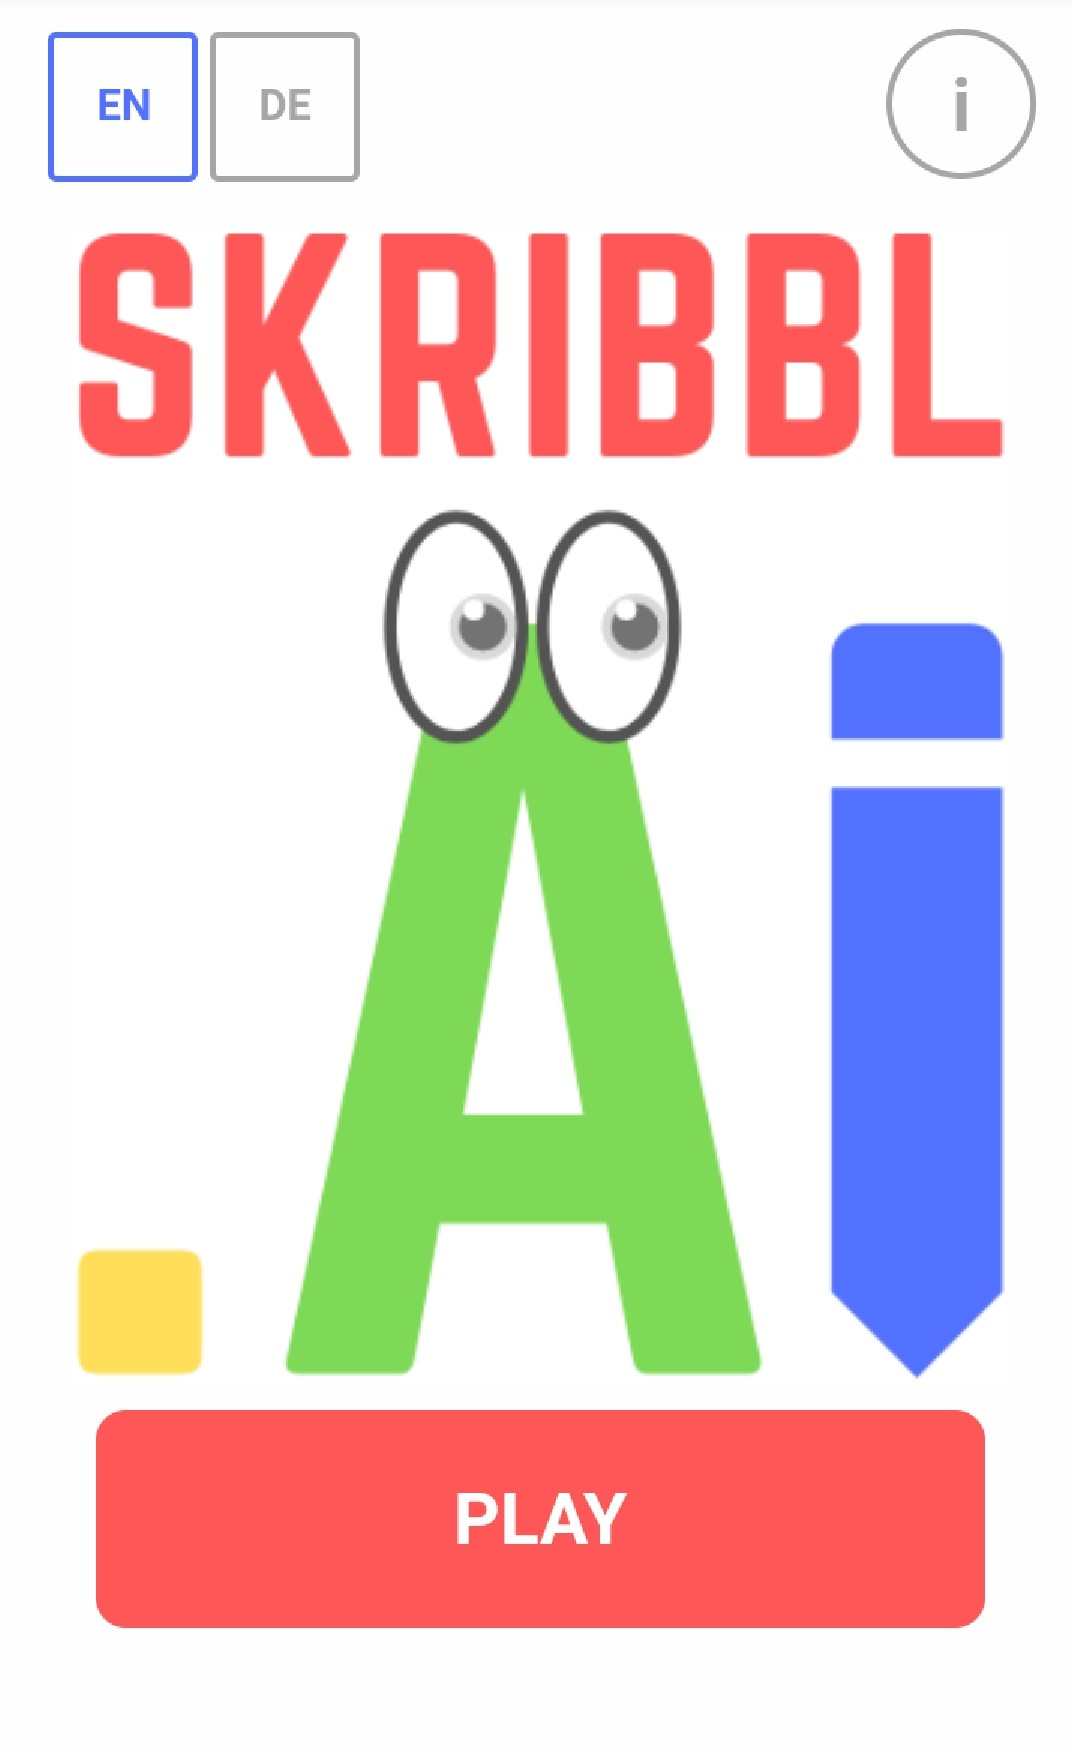
\includegraphics[width=0.25\textwidth]{images/Startscreen.jpg}
\caption{\label{fig:Startscreen}Start Bildschirm}
\end{wrapfigure}

Einen Großteil unseres Startscreens nimmt unser Logo ein. Es ist mit den vier Farben rot, grün, blau und gelb gestaltet. Beim Schriftzug 'Skribbl.Ai' ist das '.Ai' sehr groß geschrieben um besonders hervorzuheben, dass es sich hierbei um ein Spiel mit einer künstliche Intelligenz handelt. Dabei besitzt das „A“ zwei große Augen mit welchen wir unser Logo zu einer Art Maskottchen machen und es  personifizieren. Das „i“ ist ein Stift, der einen Hinweis darauf gibt, dass die Spieler*in in unserem Spiel hauptsächlich zeichnet. \\
Über dem Logo haben wir rechts einen kleinen Info-Button, der ein Popup öffnet, in welchem eine allgemeine Spielbeschreibung des Spiel zu finden ist und auch der Hinweis auf GitHubs Datenschutzverordnung verlinkt ist. 
Links oben befinden sich zwei Buttons, welche für die Auswahl zwischen der Deutschen und Englischen Sprache gedacht sind. Diese ändern die Sprache in der die Wörter zum späteren Zeichnen angegeben werden.\\
Beim auswählen wird ein Popup geöffnet, das die Spieler*in über die Umstellung informiert. Die drei Buttons wurden alle grau gehalten um sie nicht zu sehr hervorzuheben und den Fokus auf dem Logo zu halten. Bei der Auswahl der Sprache wird der dazugehörige Button blau eingefärbt, als visuelle Rückmeldung an die Benutzer*in. 
Unter dem Logo ist ein großer, roter Button angebracht, der das Spiel startet.

\subsubsection{Spielbildschirm}

\begin{wrapfigure}{R}{0.3\textwidth}
\centering
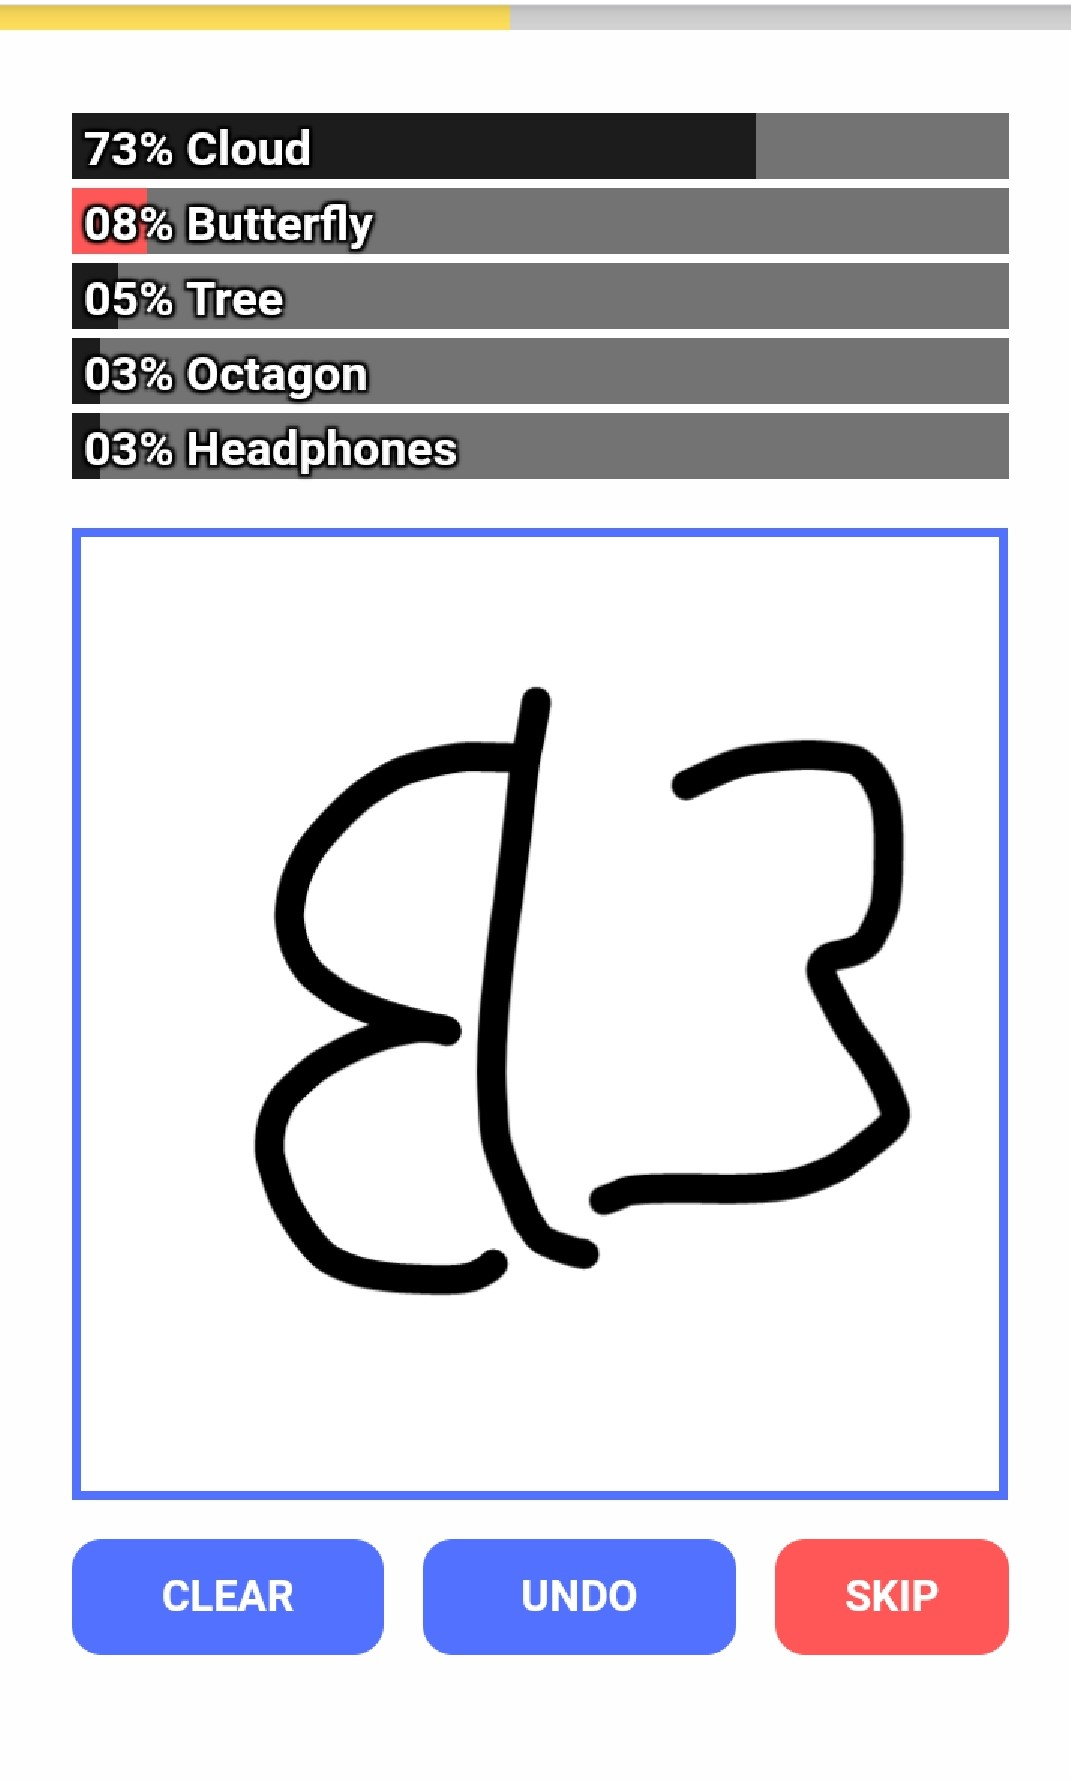
\includegraphics[width=0.25\textwidth]{images/Gamescreen.jpg}
\caption{\label{fig:Gamescreen}Spiel Bildschirm}
\end{wrapfigure}

Der Spielbildschirm ist in vier Bereiche eingeteilt. Der obere Bereich zeigt die  Zeituhr ganz oben auf der Seite. Diese ist als Balken über die gesamte Bildschirmbreite dargestellt und schrumpft von rechts nach links während sich die Farbe ändert. Der Farbverlauf geht von Grün über Gelb zu Rot. \\
Direkt unter dem Timer sieht man die Anzeige der Top fünf Wörter die die KI ausgewählt hat. Für die Anzeige der Top fünf haben wir uns sehr schnell für ein Balkendiagramm entschieden, da es für uns die beste Form der Darstellung war. Die Balken passen gut zu den anderen visuellen Elementen der Seite und sie lassen sich sehr einfach in eine Reihenfolge bringen, das \textit{Treppchensystem}. Das Balkendiagramm erstreckt sich über die gesamte Bildschirmbreite wodurch es sehr viel Platz einnimmt. Da wir für mobile Endgeräte entwickeln, muss mit dem begrenzten Bildschirmplatz sorgsam umgegangen werden. Aber da das \textit{Treppchensystem} unserer Spielidee so ein fester Bestandteil unseres Konzeptes war, überwogen die Argumente, die für die Balken sprechen. \\
Die Balken sind alle in grau gehalten, einzig wenn das zu erratende Wort als eine der Top fünf Möglichkeiten erscheint, wird dieser Balken rot gefärbt. Hiermit erkennen Spieler sehr schnell, dass sie auf einem guten Weg sind die Runde zu gewinnen. In den Balken stehen jeweils das zugehörige Wort und die Wahrscheinlichkeit der Vorhersage als Prozentzahl.\\ 
Direkt unter dem Balkendiagramm befindet sich unsere Zeichenfläche, welche blau umrandet ist.\\
Darunter sind der \textit{Clear-Button} und der \textit{Undo-Button} zu finden. Beide sind ebenfalls blau eingefärbt um zu unterstreichen, dass sie zur Zeichenfläche gehören. Rechts des \textit{Undo-Button} befindet sich der rote \textit{Skip-Button}, der eine neue Spielrunde mit einem neuen Wort startet.

Beim Tutorial wird ein Overlay über den Spielbildschirm gelegt. Hier wird ein blauer \textit{Next-Button} angeboten, der den nächsten Schritt des Tutorials zeigt, und ein roter \textit{Skip-Button}, der das Tutorial überspringt. Nach dem ersten Schritt des Tutorials, verkleinert sich das Overlay und die Beschreibung des Tutorials ist nur noch in einer kleinen grauen Box sichtbar, zu sehen in Abbildung \ref{fig:tutorial}. Somit können Spieler den Spielbildschirm und die angezeigten Elemente, die mit einer orange gestrichelten Umrandung gekennzeichnet sind, besser sehen.

\begin{figure}[ht]
\centering
    \subfigure[Tutorial: Erster Schritt]{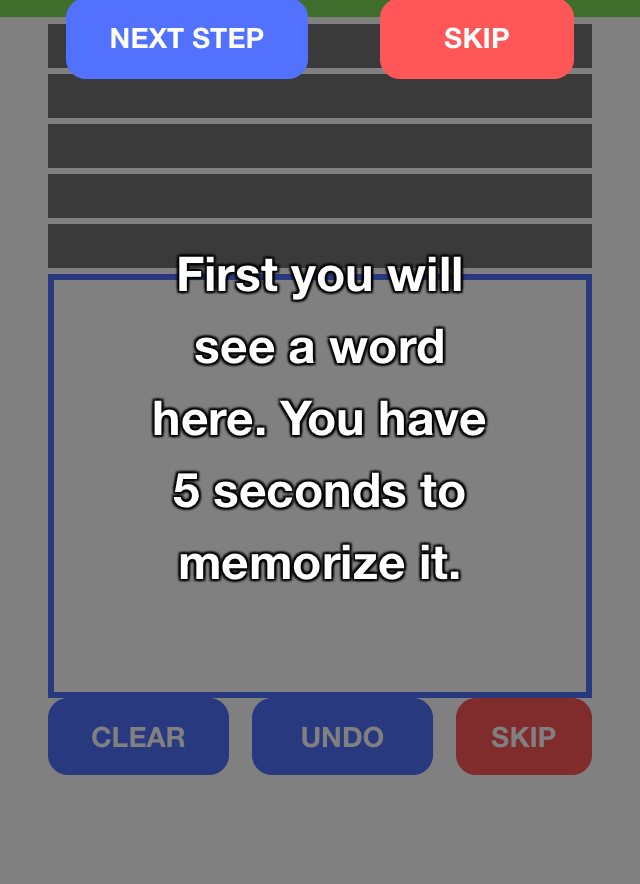
\includegraphics[width=0.3\textwidth]{images/tutorial1.png}}
    \subfigure[Tutorial: weitere Schritte]{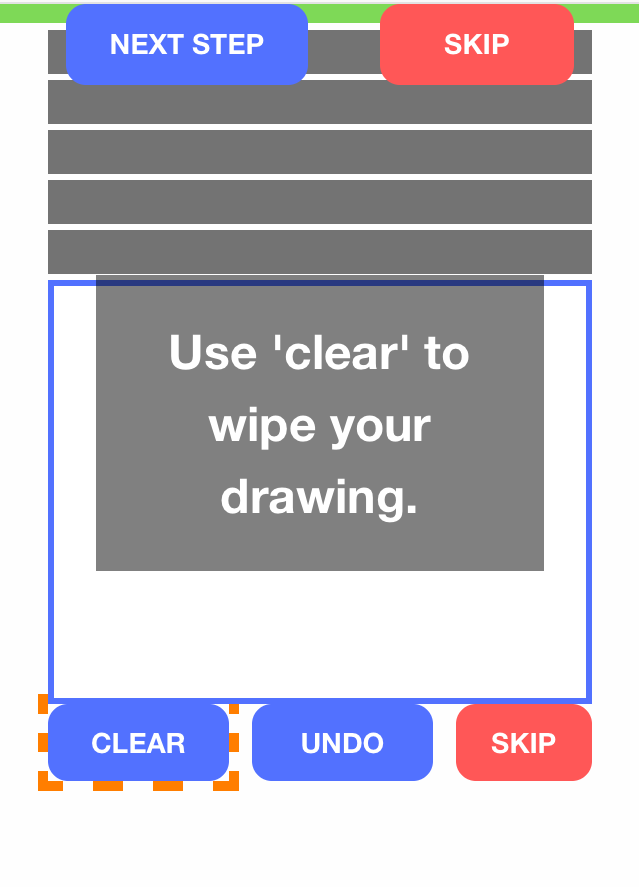
\includegraphics[width=0.3\textwidth]{images/tutorial2.png}}
\caption{\label{fig:tutorial}Tutorial Ansicht}
\end{figure}

Nach dem Tutorial, erscheint ein weiteres Overlay, welches erneut den gesamten Spielbildschirm ausgraut. Der \textit{Countdowns} und das zu zeichnende Wort befinden sich in weißer Schrift in der Mitte dieses Overlays.

\subsubsection{Endbildschirm}

Es gibt zwei verschiedene Endbildschirmansichten, der \textit{Victoryscreen} wird angezeigt, wenn die Spieler*in gewonnen hat und der \textit{Defeatscreen}, wenn das Spiel verloren wurde. Siehe hierzu Abbildung \ref{fig:endscreen}.\\
Der Aufbau dieser Ansichten unterscheidet sich nicht stark. Es wird jeweils das Logo, eine Überschrift und ein kurzer Text angezeigt. Die Texte und das Logo unterscheiden sich, je nach dem ob das Spiel gewonnen oder verloren wurde. \\
Auf dem \textit{Victoryscreen} erscheint eine Version unseres Logo in dem es so erscheint, als würde das Maskottchen sich freuen und feiern. Eine große rote Überschrift informiert den Spieler, dass er gewonnen hat. Daneben steht ein Text welcher die Spieler*in über ihre Prozentzahl und die benötigte Zeit informiert.\\
Der \textit{Defeatscreen} hingegen zeigt eine Version unseres Logos, auf dem es aussieht, als würde es Weinen und sich mit der Spieler*in ärgern. Hier wird angezeigt welches Wort an oberster Stelle stand und mit welcher Prozentzahl. Die rote Überschrift informiert hier zusätzlich noch, dass die Zeit abgelaufen war.\\
Unter Logo und Text befindet sich in beiden Ansichten das Bild, welches gezeichnet wurde. Unter der Zeichung befinden sich zwei Knöpfe. Rechts ist ein roter \textit{Next-Button}, der zur nächsten Spielrunde führt und links ein blauer \textit{Menü-Button}, der zurück zur Startseite führt.

\begin{figure}[ht]
\centering
    \subfigure[VictoryScreen]{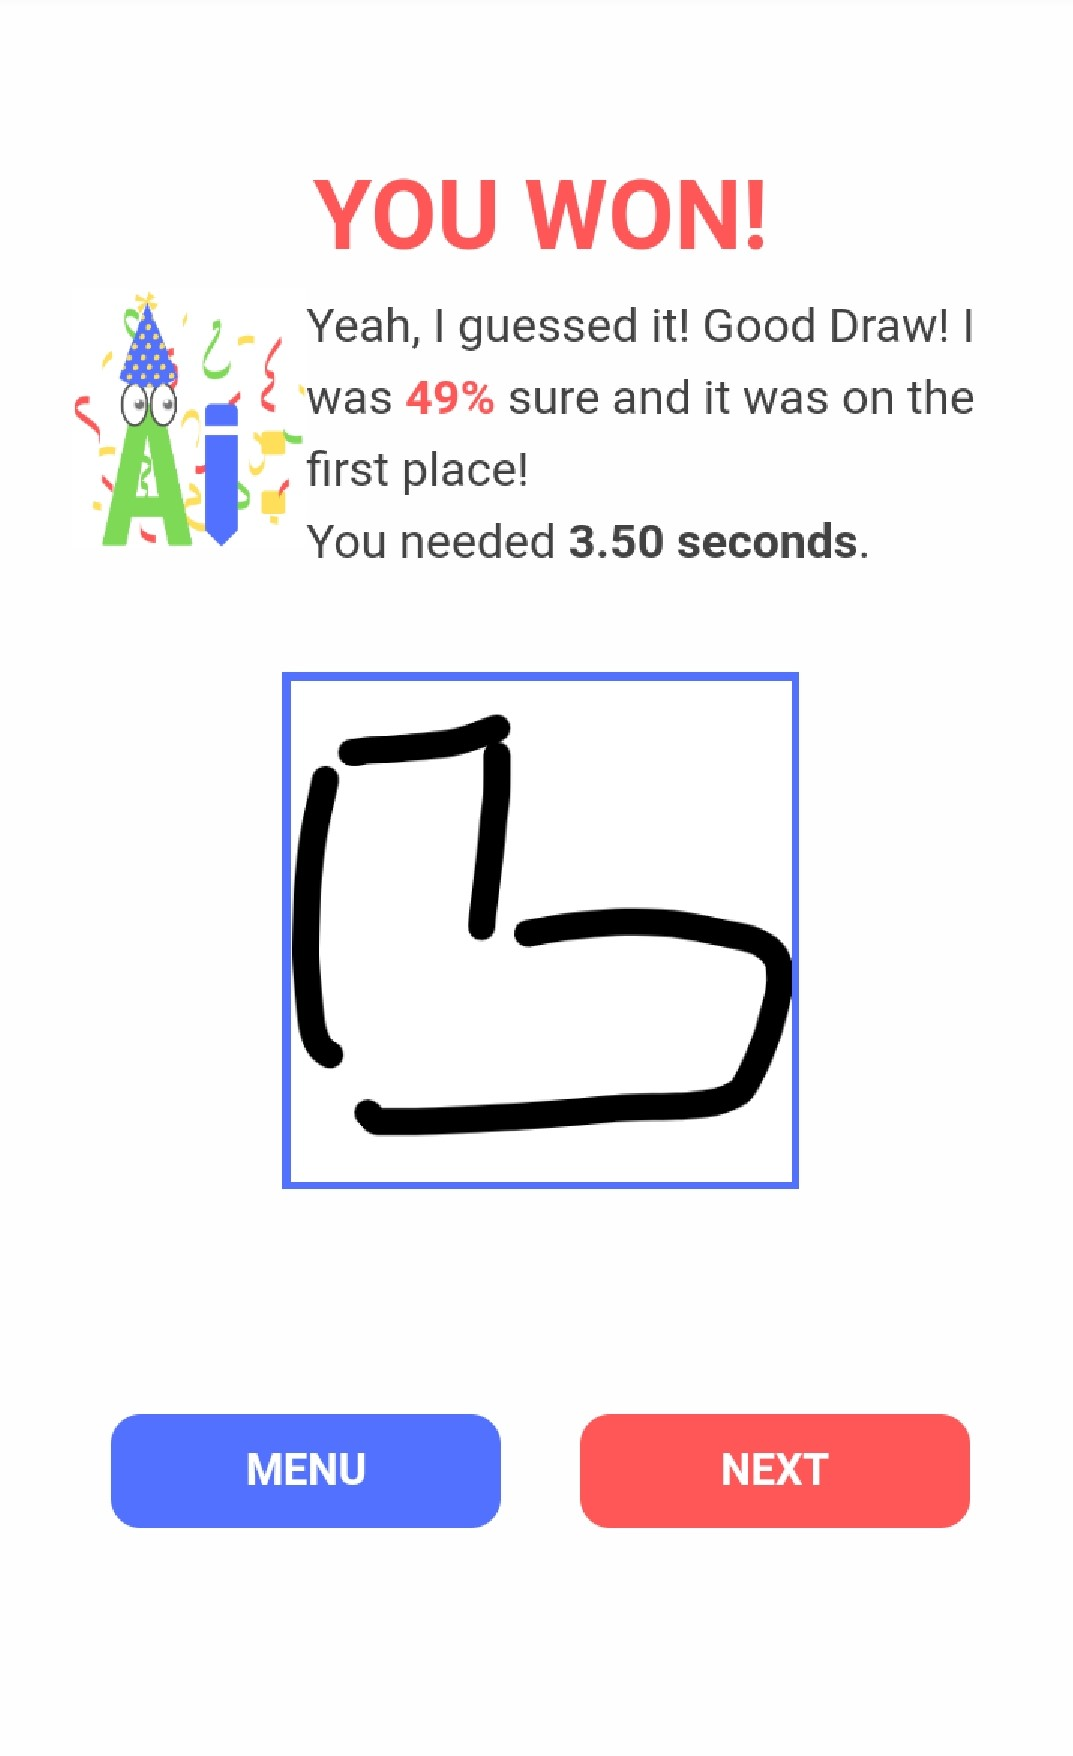
\includegraphics[width=0.3\textwidth]{images/Victoryscreen.jpg}}
    \subfigure[DefeatScreen]{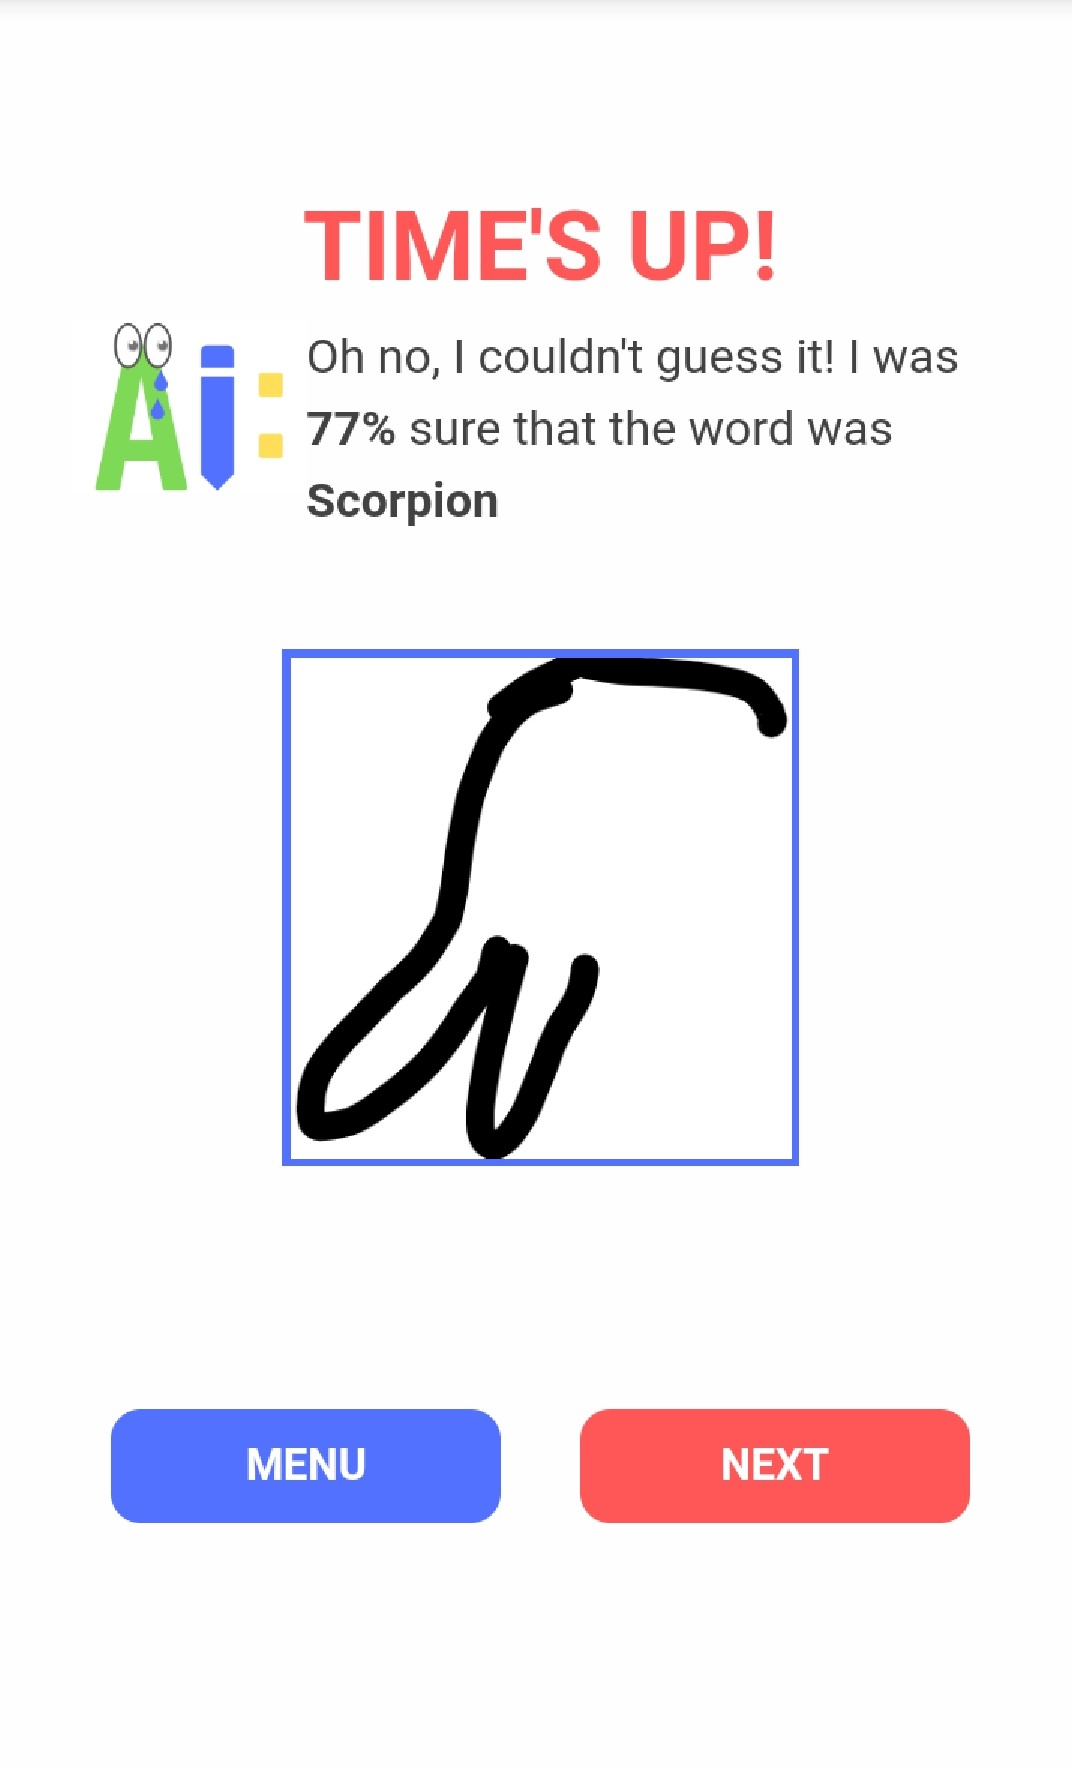
\includegraphics[width=0.3\textwidth]{images/Defeatscreen.jpg}}
\caption{\label{fig:endscreen} Endbildschirm}
\end{figure}

\subsection{Künstliches neuronales Netzwerk}

Künstliche Intelligenz beschäftigt sich mit den Möglichkeiten Aufgaben zu lösen und zu automatisieren, die normalerweise von Menschen bearbeitet werden. Dabei ist maschinelles Lernen eine Untermenge der künstlichen Intelligenz. Künstliche neuronale Netze stellen wiederum eine Teilmenge des maschinellen Lernens dar. Künstlichen neuronale Netze versuchen auf einfacher Weise das menschliche Gehirn abzubilden. Dabei werden die Strukturen dem biologischen Vorbild nachempfunden. Einzelne Nervenzellen werden als Knoten abstrahiert, die Verbindungen der Nervenzellen (Axon) werden durch Verbindungen beziehungsweise Kanten der Knoten realisiert. Künstliche neuronale Netze sind in der meisten Fällen so aufgebaut, dass es einen \textit{Eingangslayer}, bestehend aus ein oder mehreren Knoten, gibt, sowie einen oder mehreren versteckten \textit{Layern}. Nach den versteckten \textit{Layer(n)} folgt der \textit{Ausgangslayer}. Dieser beinhaltet die Ausgangsknoten. Die einzelnen Knoten und \textit{Layer} sind durch Kanten miteinander verbunden. Jede dieser Kanten wird ein Gewicht zugewiesen und jedem Knoten im Netzwerk eine Aktivierungsfunktion. Entsprechend dem biologischen Vorbild leitet ein Knoten das Eingangssignal weiter, wenn die Eingangssignale einen entsprechenden Schwellwert, bestimmt durch die Aktivierungsfunktion, überschreiten.

Künstliche neuronale Netze werden meist für Klassifizierungsaufgaben verwendet. Demnach enthält der \textit{Ausgangslayer} für jede Klasse einen entsprechenden Knoten der für die entsprechende Klasse steht. Die Aktivierungslevel der Ausgangsknoten geben Auskunft über das Ergebnis der Klassifizierung.  Damit ein künstliches neuronales Netz (KNN) eine Aufgabe lösen kann, gilt es die Gewichte der Kanten und die Parameter der Aktivierungsfunktionen dahingehend zu optimieren, dass die Ausgangswerte sich möglichst nahe an die erwarteten Werte anpassen. Dieser Vorgang wird als Lernen bezeichnet.

Ziel des Lernens ist es, ein Modell zu schaffen, welches die Beziehung zwischen den Eingangs- und den Ausgangsdaten eines Systems möglichst genau beschreibt. Um diesen Prozess zu ermöglichen und das Lernen des KNN durchzuführen ist eine entsprechende Menge an Daten erforderlich.\parencite{M.AnderssonM.Arvola}\parencite{Chollet2017}

\subsubsection{Trainieren eines Netzwerkes}

Damit das Netzwerk die Beziehungen zwischen Eingangs- und Ausgangsdaten beschreiben kann, wird das Netz mit dem vorhandenen Daten trainiert. Für das Trainieren beziehungsweise Lernen eines KNN gibt es verschiedene Vorgehensweisen. Zum Einen gibt es das sogenannte \textit{Supervised Learning}, bei dem der Datensatz für das Training bereits klassifiziert vorliegt. Dem gegenüber steht die Methode des \textit{Unsupervised Learning}.

\paragraph{Supervised Learning}
Beim \textit{Supervised Learning} ist jedem Datensatz ein \textit{Label}, auch Klasse, zugewiesen. Das Netzwerk wird mit zufälligen Parametern initialisiert und es wird versucht die Parameter so anzupassen, dass die Ausgangsneuronen das erwartete Ergebnis liefern. Während des Lernens, werden die Parameter des Netzes dahingehend optimiert, dass die Abweichung der Ausgangsneuronen zu dem gewünschten Ergebnis minimiert wird.\parencite{Pattanayak2017}

\paragraph{Unsupervised Learning}
Beim \textit{Unsupervised Learning} sind dem Lerndatensatz keine \textit{Labels} oder Klassen zugewiesen. Algorithmen dieser Kategorie zielen auf Strukturen innerhalb des Lerndatensatzes ab. Während des Lernens entstehen \textit{Cluster}, die einer Klassifizierung entsprechen.\parencite{Pattanayak2017}

\subsubsection{Aktivierungsfunktionen}
Der Gedanke hinter Aktivierungsfunktionen ist die Nachbildung des Verhaltens menschlicher Nervenzellen. Ab einem bestimmten Schwellwert, auch Aktivierungspotential  genannt, wird das Neuron aktiv, das heißt es beginnt zu feuern. Das bedeutet, das Neuron leitet sein Signal weiter. Aktivierungsfunktionen sollen die Ausgabe in einem kleinen Wertebereich (meist -1 bis 1) liegen.\parencite{Manaswi2018}

\paragraph{ReLU Aktivierungsfunktion}
Die \textit{Rectified Linear Unit} (ReLU) ist eine Aktivierungsfunktion, die aufgrund ihrer Einfachheit und Leistungsfähigkeit, immer beliebter wird. Für negative Eingangswerte wird die Funktion null, für alle positiven Werte nimmt die Funktion den Eingangswert an.\parencite{M.AnderssonM.Arvola}

\paragraph{SoftMax Aktivierungsfunktion}
Bei Klassifizierungsproblemen sollte das Ergebnis für die entsprechende Klasse stehen beziehungsweise für die Wahrscheinlichkeit der Zugehörigkeit zu einer Klasse. Durch Verwendung der SoftMax Funktion im \textit{Ausgabelayer} liegen die Ausgabewerte zwischen null und eins, diese können entsprechend als Klassenwahrscheinlichkeit interpretiert werden. Hierfür haben auch wir diese Funktion verwendet. \parencite{LindholmWahlstromLindsten2019}

\subsubsection{Convolutional Neural Network}
Ein \textit{Convolutional Neural Network} nutzt Faltungsoperatoren beziehungsweise Faltungsschichten (\textit{Convolution Layer}) um Merkmale aus Bildern zu extrahieren. Im Rahmen des Projektes kommen sogenannte \textit{2D-Convolution Layern} zum Einsatz. Diese nutzen 2D Faltungsoperatoren zur Merkmalsextraktion. Durch das Training werden diese Operatoren gelernt. Beispielsweise können so bekannte Filter, wie Kantendetektoren oder Weichzeichner enstehen. Somit lernt das neuronale Netz Bildverarbeitungsfilter die bekannten Filtern ähneln oder sich stark von diesen unterscheiden. Im Allgemeinen lernt der erste \textit{Convolution Layer} einfache Merkmale, beispielsweise Kanten, zu erkennen. Darauffolgende Schichten lernen darauf aufbauend immer komplexer werdende Merkmale zu extrahieren. Ein Vorteil eines CNN ist die geringe Anzahl an Parametern.\parencite{Pattanayak2017}

\paragraph{Fully Connected Layer}
In einem sogenannten \textit{Fully Connected Layer}, auch \textit{Dense Layer} genannt, sind alle Neuronen oder Knoten mit den Neuronen des vorhergehenden oder nachfolgenden Layer verbunden.\parencite{Pattanayak2017}

\paragraph{Pooling Layer}
\textit{Pooling Layer} dienen der Verdichtung von Daten. Dies tun sie indem sie Bereiche von Ausgabedaten mit Hilfe von statistische Operationen zusammenfassen. Dies dient der Reduktion von Parametern und der Vereinfachung von Berechnungen.  \textit{Max Pooling Layer} sind eine der am häufigsten eingesetzten Arten von \textit{Pooling Layern} und kommen auch im Rahmen dieses Projektes zum Einsatz. Sie reduzieren eine Region, indem sie nur den Maximalwert der Region erhalten. \textit{Pooling Layer} folgen meist auf \textit{Convolution Layer}.\parencite{Karpathy}\parencite{IanGoodfellowYoshuaBengio2016}

\section{Anforderungen}
\label{chap: Anforderungen}
\subsection{Produkt Vision}
\label{chap: productVision}
Unsere Produkt Vision ist es, bis zum Ende des Wintersemesters 2018/2019 ein kurzweiliges Mini-Malspiel mit einem Einzelspielermodus entwickelt zu haben. Es soll speziell für mobile Endnutzer aller Altersklassen konzipiert sein.
\subsubsection{Die Kurzweiligkeit}
Die Kurzweiligkeit unseres Spiels ist offensichtlich eine der Eigenschaften, die am schwierigsten einzuschätzen sind. Um dennoch dieses Ziel nicht aus den Augen zu verlieren, einigten wir uns darauf, alle Tickets, Erweiterungen und Ideen, die sich mit dem Spielkonzept beschäftigen würden, auf ihren Unterhaltungswert zu prüfen.
\subsubsection{Das Mini-Spiel}
Das Spiel sollte rundenbasiert sein und jede Runde sollte nur wenige Minuten dauern. Damit wollen wir gewährleisten, dass es gut als Zeitvertreib während beispielsweise dem Fahren öffentlicher Verkehrsmittel oder dem Warten in der Schlange eines Coffeeshop gespielt werden kann. Konkret sollte eine Runde nicht länger als zwei bis drei Minuten dauern.
\subsubsection{Das Mal-Spiel}
Um das Spiel zu spielen, wird die Spieler*in als Hauptaufgabe Zeichnen. Dabei sollen übliche Werkzeuge wie ein \textit{undo}-Knopf, zum Entfernen des zuletzt gemalten Strichs und ein \textit{clear}-Knopf, zum Entfernen der gesamten Zeichnung, implementiert werden. Weiter wird die Spieler*in direkt mit dem Finger auf dem Bildschirm beziehungsweise mit Hilfe der Maus Zeichnen können. Mehr dazu in Kapitel \ref{chap:spielkonzept}.
\subsubsection{Der Einzelspielermodus}
Skribbl.AI soll von einer einzelnen Person gespielt werden können. Über Gewinn oder Verlust soll die vergangene Zeit entscheiden, welche die Spieler*in benötigt haben wird, um das geforderte Wort zeichnerisch darzustellen. Mehr hierzu ebenfalls in Kapitel \ref{chap:spielkonzept}.
\subsubsection{Für mobile Geräte}
Um Skribbl.AI auf vielen verschiedenen mobilen Endgeräten spielen zu können ohne verschiedene Programme für unterschiedliche Betriebssysteme entwickeln zu müssen, entschieden wir uns für eine webbasierte Anwendung. Das Spiel sollte dann auf einem, über das Internet erreichbaren Host, veröffentlicht werden, sodass es umstandslos mit üblichen Browsern gespielt werden kann.
\subsubsection{Für alle Altersklassen}
Das Spiel sollte für alle Alterklassen interessant und spielbar sein. Neben der Eigenschaft, dass eine Runde nur eine bestimmte Dauer haben sollte, würden hier hauptsächlich die Begriffe, die die Spieler*in malen sollte, ausschlaggebend sein. Siehe hierzu Kapitel \ref{chap:spielkonzept}.
\subsection{Spielkonzept}
Um die, in Kapitel \ref{chap: productVision} genannten Eigenschaften in unserem Spiel umzusetzen entwarfen wir verschiedene Spielkonzepte. Das Konzept, auf welches wir uns letzendlich einigten sieht wie folgt aus.
Die Spieler*in sollte zu Beginn einer Spielrunde für wenige Sekunden ein Wort aus einem Pool von Wörtern gezeigt bekommen. Dieses Wort ist dann innerhalb eines festgelegten Zeitraums zu Zeichnen.

Die optimale Zeit, die eine Runde andauern sollte, würde im späteren Verlauf des Projekts ermittelt werden. Hierzu haben alle Teammitglieder insgesamt 24 verschiedene Begriffe gezeichnet und dabei die Zeit, die gebraucht wurde bis das Wort erkannt wurde (oder das Teammitglied aufgab) festgehalten. Mit Hilfe der Ergebnisse, ein Ausschnitt dieser ist zu sehen in Abbildung \ref{fig:testResults}, bestimmten wir einen Durchschnitt, der angebrachte Zeit darstellte. 

\label{chap:spielkonzept}
\begin{figure}[ht]
\centering
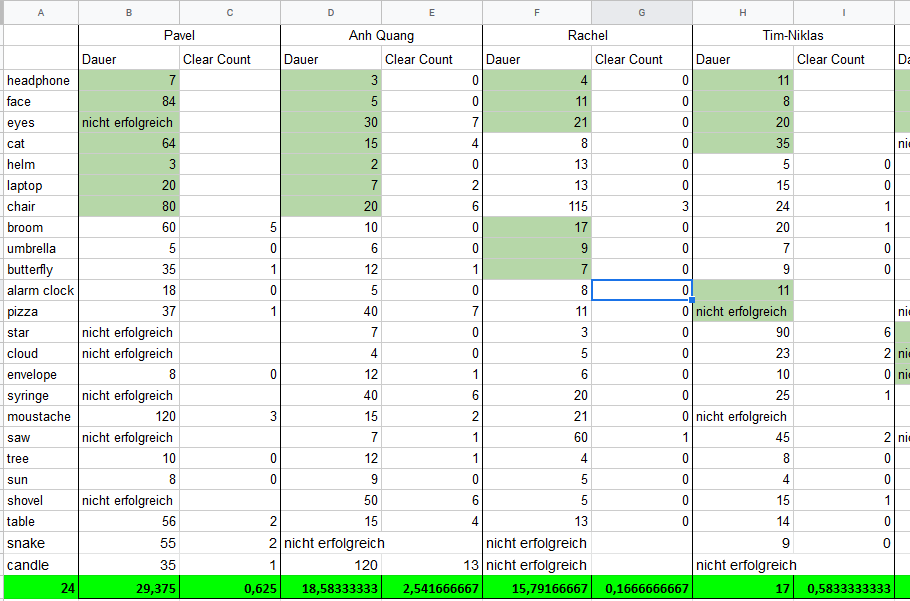
\includegraphics[width=1\textwidth]{images/blindtesting.png}
\caption{\label{fig:testResults}Ergebnisse des Testzeichnen}
\end{figure}

Jedes Mal wenn die Spieler*in "den Stift absetzt", das bedeutet in unserem Fall, den Finger hebt um neu anzusetzen, soll das gezeichnete Bild an das neuronale Netzwerk übergeben werden. Dieses berechnet dann die Ergebnisse. Die fünf Ergebnisse mit den höchsten Vorhersagewahrscheinlichkeiten sollen auf dem Spielbildschirm angezeigt werden. Für die Anzeige eben jener fünf wahrscheinlichsten Wörter soll ein Balkendiagramm verwendet werden, welches das Wort und die zugehörige Wahrscheinlichkeit in Prozent zeigt. Außerdem soll, falls das korrekte Wort in der Auswahl enthalten ist, dieses farblich hervorgehoben werden. Am oberen Rand des Spielbildschirms soll ein farblich gestalteter Balken anzeigen, wie viel Zeit schon vergangen ist. Wenn die Spieler*in es schafft, eine  Zeichnung innerhalb der vorgegebenen Zeit zu erstellen und das neuronale Netzwerk diese als das vorgegebene Wort erkennt, dann ist die Runde gewonnen. Dies bedeutet, dass das gesuchte Wort in den Vorhersagen des neuronalen Netzwerks die höchste Wahrscheinlichkeit verglichen mit allen anderen Möglichkeiten haben muss. Verloren ist das Spiel, wenn dies der Spieler*in nicht in der vorgegebenen Zeit gelingt. 
In beiden Fällen hat die Spieler*in schließlich die Möglichkeit eine neue Runde mit einem neuen Wort zu starten.

\section{Implementierung}
\subsection{JavaScript}
Für die Architektur orientierten wir uns grob am Model View Controller Design Pattern.
\subsubsection{Methodik}
Um eine sinnvolle Architektur für Skribbl.AI zu entwerfen wurde die Class-Responsibility-Collaboration Card Methode verwendet. Zu sehen in Abbildung \ref{fig:crcCard}. Zunächst wurden mit Hilfe des bereits existierenden Programmcodes Klassen definiert und anschließend die jeweiligen Verantwortlichkeiten und Kollaborationen mit anderen Klassen notiert. Das Resultat dieser Überlegung wurde daraufhin in Programmcode übersetzt und ist in der folgenden Abbildung zu sehen.

\begin{figure}[ht]
\centering
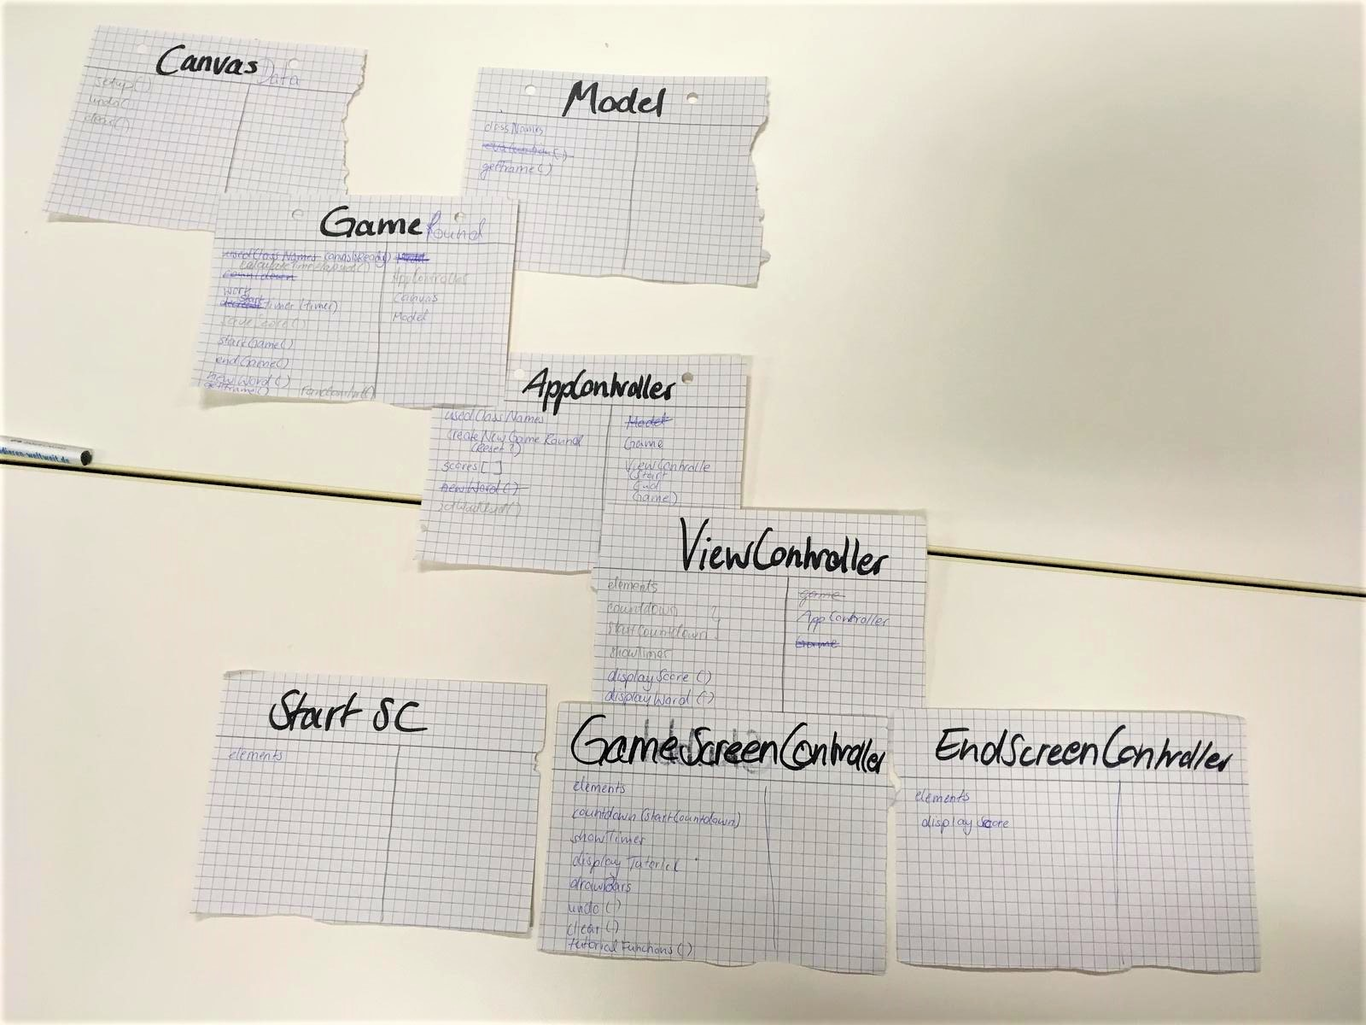
\includegraphics[width=0.75\textwidth]{images/crc.png}
\caption{\label{fig:crcCard}\textit{Class Responsibility Collaborator} Karten}
\end{figure}

\subsubsection{Das Model}
Die Klassen des \textit{Model} sind in Abbildung \ref{fig:classDiagram} blau hinterlegt. Die \textit{CanvasData} Klasse ist zuständig für die Speicherung und Verarbeitung der Daten die auf dem \textit{Canvas} entstehen. Dazu gehören beispielsweise die Maus Koordinaten und das Zuschneiden des gemalten Bildes auf die passende Größe. Die \textit{ModelData} Klasse bindet das neuronale Netzwerk ein und berechnet die Vorhersagen. Die \textit{GameRound} Klasse wiederum speichert alle Informationen zur aktuellen Spielrunde wie die übrige Zeit und das aktuelle Wort. Die Klassen \textit{Tutorial} und \textit{TutorialStep} sind für die Steuerung durch das Tutorial und die Hervorhebung der betreffenden Bildschirmbereiche verantwortlich. Die \textit{Score} Klasse speichert die Gewinninformationen der Runde.

\subsubsection{Der Applikation Controller}
Die Klasse \textit{AppController} steuert den Verlauf des Spiels. Sie weiß in welchem Status das Spiel sich befindet, welche Wörter bereits benutzt wurden und kann neue Runden starten. Da wir für unsere Applikation immer nur einen \textit{AppController} benötigen ist dieser als \textit{Singleton} implementiert. Hierfür wird eine Instanz der Klasse \textit{AppController} in der Klasse \textit{SingletonAppController} gekapselt. Die Klasse \textit{SingletonAppController} ist nur dafür zuständig zu prüfen, ob bereits eine Instanz von \textit{AppController} existiert und gegebenenfalls eine Neue zu erstellen oder die Existierende zurück zu geben. \textit{AppController} und \textit{SingletonAppController} sind in Abbildung \ref{fig:classDiagram} grün hinterlegt.

\subsubsection{Der View Controller}
Es gibt eine \textit{ViewController} Klasse, diese initialisiert den \textit{AppController} als Feld. Von dieser Klasse erben die Klassen \textit{StartScreenController}, \textit{GameScreenController} und \textit{EndScreenController}, alle vier Klassen sind in Abbildung \ref{fig:classDiagram} rot hinterlegt. Die Kindklassen repräsentieren jeweils einen Spielstatus und sind zuständig die korrekten Bildschirmbereiche anzuzeigen und die dazugehörigen Funktionalitäten zur Verfügung zu stellen. Hierzu gehören die Spracheinstellung auf dem Startbildschirm oder \textit{undo} und \textit{clear} auf dem Bildschirm des Hauptspiels.

\begin{figure}[ht]
\centering
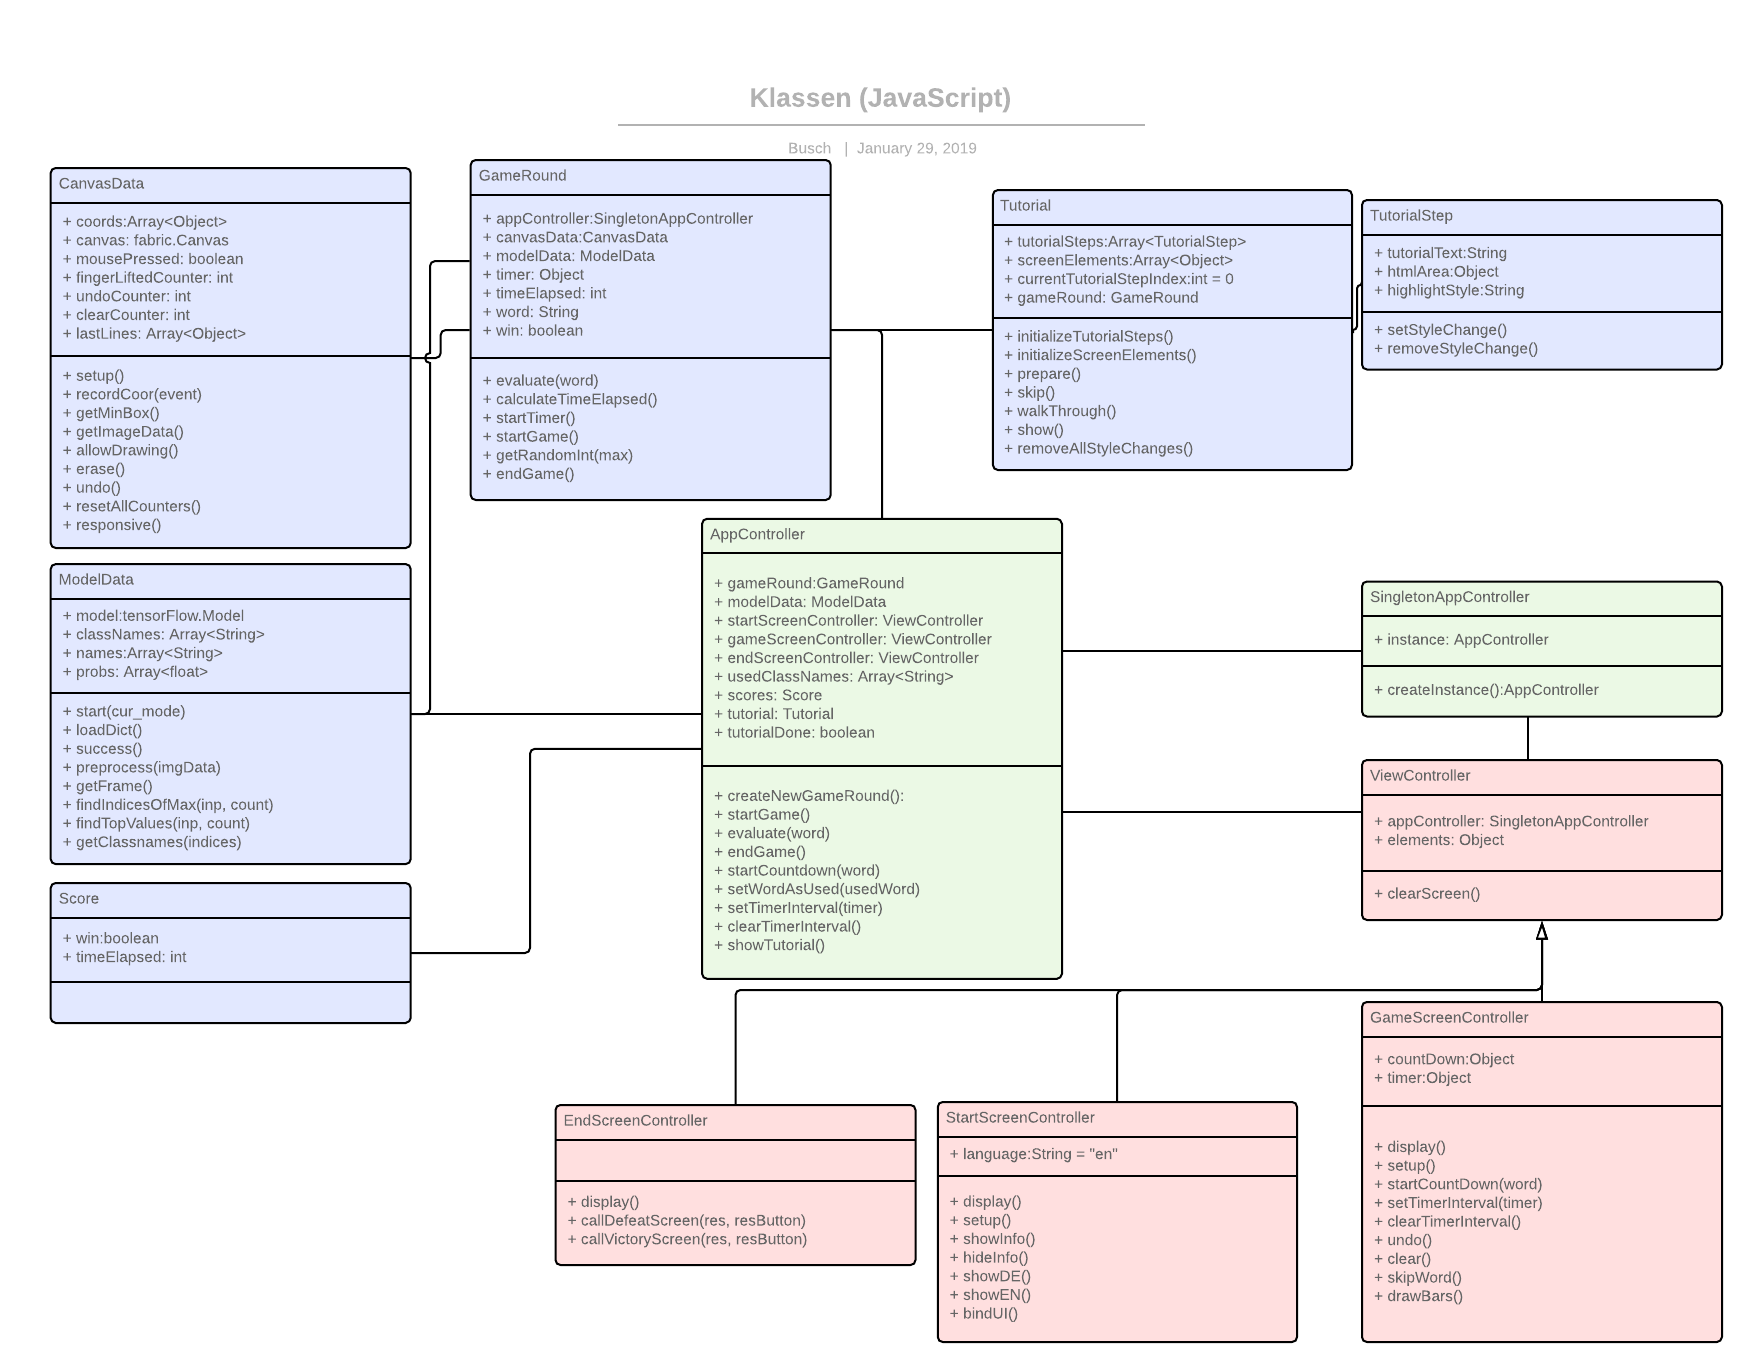
\includegraphics[width=1\textwidth]{images/classDiagramSkribbl.png}
\caption{\label{fig:classDiagram}Klassen Diagramm}
\end{figure}

\newpage
\subsection{Neuronales Netz}
\subsubsection{Datensatz}
Der Datensatz mit dem das künstliche neuronale Netz trainiert wurde, wird von \textit{Google} bereit gestellt. Dieser basiert auf dem Spiel \textit{Quick, Draw!} und beinhaltet eine Vielzahl verschiedener Klassen.  Zudem wurden im Rahmen dieses Spiels weitere Daten gesammelt. Der Datensatz beinhaltet viele verschiedene Skizzen zu verschiedenen Begriffen. Es sind meist einfache Strichzeichnungen die von Spielern im Rahmen dieses Spiels angefertigt wurden. Bei dem Spiel geht es darum, einen vorgegebenen Begriff durch einer Skizze darzustellen. Aktuell beinhaltet der Datensatz 345 Kategorien, mit mehr als 50 Millionen Zeichnungen. Der Datensatz steht im verschiedenen Formaten zur Verfügung.
Für die Projektarbeit wurden der Datensatz im Form der .npy Dateien verwendet. Das .npy-Format liefert die Skizzen mittig ausgerichtet und in der Größe von 28x28 Pixeln als Graustufenbilder.\parencite{GoogleCreativeLab2018}
Im Rahmen dieser Projektarbeit wurden 100 Kategorien mit jeweils 20.000 Bildern für das Modell ausgewählt.

\subsubsection{Aufbau des Netzes}
Für die Umsetzung des KNNs wurde die Open-Source-Softwarebibliothek \textit{Tensorflow} verwendet. Zusätzlich wurde \textit{Keras} als API für den Zugriff auf \textit{Tensorflow} in Python 3.0 verwendet. Dabei stellt \textit{Keras} eine \textit{high level} API, da die \textit{Tensorflow} im Hintergrund verwendet. \textit{Keras} bietet verschiedene Typen von Layern, Aktivierungsfunktion, vortrainerte Modelle und weitere Funktionen an.

Der Trainingsdatensatz für das Modell besteht aus 100 Klassen mit je 20.000 Skizzen. Dieser wurde aufgeteilt in Trainingsdaten (80\%) und Testdaten (20\%).

Für die Lösung der Aufgabe innerhalb dieser Projektarbeit sollte  ein \textit{Convolutional Neural Network} (CNN) verwendet werden. Dieser besondere Typ eines KNNs nutzt sogenannte Faltungsschichten (\textit{Convolution Layers}) zur Vorverarbeitung der Daten innerhalb des Netzes.
Das Design des verwendeten Netzes enthält drei 2D-Convolutional Layern, die alle die ReLU Aktivierungsfunktion verwenden. Auf jeden \textit{Convolutional Layer} folgt ein \textit{Max Pooling Layer}. Aufgabe dieser Layer ist die Reduktion der Parameter. Anschließend folgt ein \textit{Fully Connected Layer} mit 128 Knoten und der ReLU Aktivierungsfunktion als \textit{Hidden Layer}. Zum Abschluss folgt der Ausgabelayer mit 100 Knoten und SoftMax Aktivierungsfunktion.

Das Modellieren eines neuronales Netzes stellt sich in der Regel als sehr komplexes Thema dar. Zudem existieren bereits viele Modelle für verschiedenste Aufgaben als Ergebnisse unterschiedlichste Studien. Viele von diesen sind im Internet frei verfügbar. Nachdem wir verschiedene einfache Modelle probiert und getestet haben, haben wir uns schließlich für das Modell von Zaid Alyafeai\parencite{ZaidAlyafeai2018} entschieden. Alyafeai erreichte in seinem Versuchen mit diesem Aufbau eine Genauigkeit von ca. 92,20\%. Dabei verwendete er 5.000 Datensätze pro Klasse. Wir konnten eine Genauigkeit von   94,69\% erreichen unter Verwendung von 20.000 Datensätze pro Klasse.

Für die Verbesserung der Genauigkeit wurden verschiedene Parameter variiert. Zuerst wurde die Anzahl der Trainingsdaten schrittweise von 5.000 auf 20.000 erhöht. Anschließend wurden die Epochen während des Trainings weiter angehoben (von 5 auf 15). 
Zusätzlich zu dem automatischen Tests nach dem Lernprozess, wurden die einzelnen entstandenen Netze auch manuellen Tests unterzogen.

\section{Spielbeschreibung, Ziel}

\iffalse
Spielkonzept ist bereits beschrieben in Anforderung, Spielkonzept
\fi

\section{Bewertung}
vgl. Anforderungen mit Ergebnis
\pagebreak

\pagenumbering{Roman}
\section{Anlangen}
\label{chap: Anlagen}
\subsection{Styleguide}


\textbf{Generelle Regeln}
\begin{itemize}
\item Daten sollten so gut wie möglich und so oft wie möglich in Diagrammen und Bildern dargestellt werden
\item Text sollte bis zu 200\% vergrößert werden können
\item Bilder sollten einen Alt-Data Text haben
\end{itemize}

\textbf{Knöpfe}
\begin{itemize}
\item Sollen einen ausreichenden Farbkontrast haben (Kontrast nach Web Content Accessibility Guidelines 2 AA \parencite{Caldwell2008})
\item Texte auf \textit{Buttons} sollen kurz und schlüssig formuliert werden
\item Abkürzungen gerne, aber sie sollen entweder aus einem Idiom bestehen oder einmal erklärt worden sein
\end{itemize}

\textbf{Formattierung}
\begin{itemize}
\item Klammerpaare sollen vertikal immer aneinander ausgerichtet sein
\item \textit{if, while} und \textit{for} Anweisungen müssen immer mit Klammern geschrieben werden, auch wenn sie nur eine Kondition aufweisen
\item Binäre Operatoren sollen ein Leerzeichen auf jeder Seite haben
\item Klammern sollen in Ausdrücken verwendet werden um Klarheit und Einfachheit im Code zu verbessern
\item Klassennamen starten mit einem Großbuchstaben (Binnenmajuskeln sind erlaubt wenn notwendig)
\item Alle anderen Identifikatoren starten klein geschrieben und benutzen daraufhin Binnenmajuskeln (keine Leerzeichen)
\end{itemize}

\textbf{Coding}
\begin{itemize}
\item Jede Methode sollte etwas zurück geben
\item Es wird kein \textit{Continue} benutzt
\item \textit{break} wird nicht außerhalb eines \textit{switch-cases} benutzt
\item Variablen werden so nahe wie möglich am Ort ihrer Benutzung initialisiert
\item Öffentliche Variablen so wenig wie nötig benutzen
\end{itemize}

\textbf{Farben}

\begin{tabular}{llll}
\#7ED957    Grün & \#FF2E2E    Rot & \#4265FF    Blau & \#FFDE59    Gelb \\
\#545454    Dunkleres Grau & \#737373    Dunkle Grau & \#A6A6A6    Helles Grau & \#D9D9D9    Helleres Grau\\
\end{tabular}
\pagebreak

\begin{large}\textbf{Schrift}\end{large}
\begin{itemize}
\item Schriftgröße: Entweder 18 px oder 14 px und fett (Je nach Media Queries und Layout)
\item Schriftstyle: non-serif, non-monospace
\item Schriftart: Standard Browser Schriftart und Norwester für das Logo
\end{itemize}

\textbf{Sprache}
\begin{itemize}
\item Einfache Sprache
\item English/Deutsch(für die zu zeichnenden Wörter)
\end{itemize}

\pagebreak
\printbibliography
\end{document}
